\section{Future Work}
In the future we would like to attempt 3 things, the first being to train on even more games. There are approximately 4.5 trillion board states and we trained over at most 3.78 million. We think that the filters may not have been fully trained resulting in worse performance. 

Another step we would like to try is to adjust the network structure. Currently we are passing the valid moves to the convolution layer. We think that merging the valid moves with the output of the dense layer $lout$ allow it to pick better moves faster. This change would make the network structure look like Figure \ref{fig:struct_future}.

\begin{figure}
  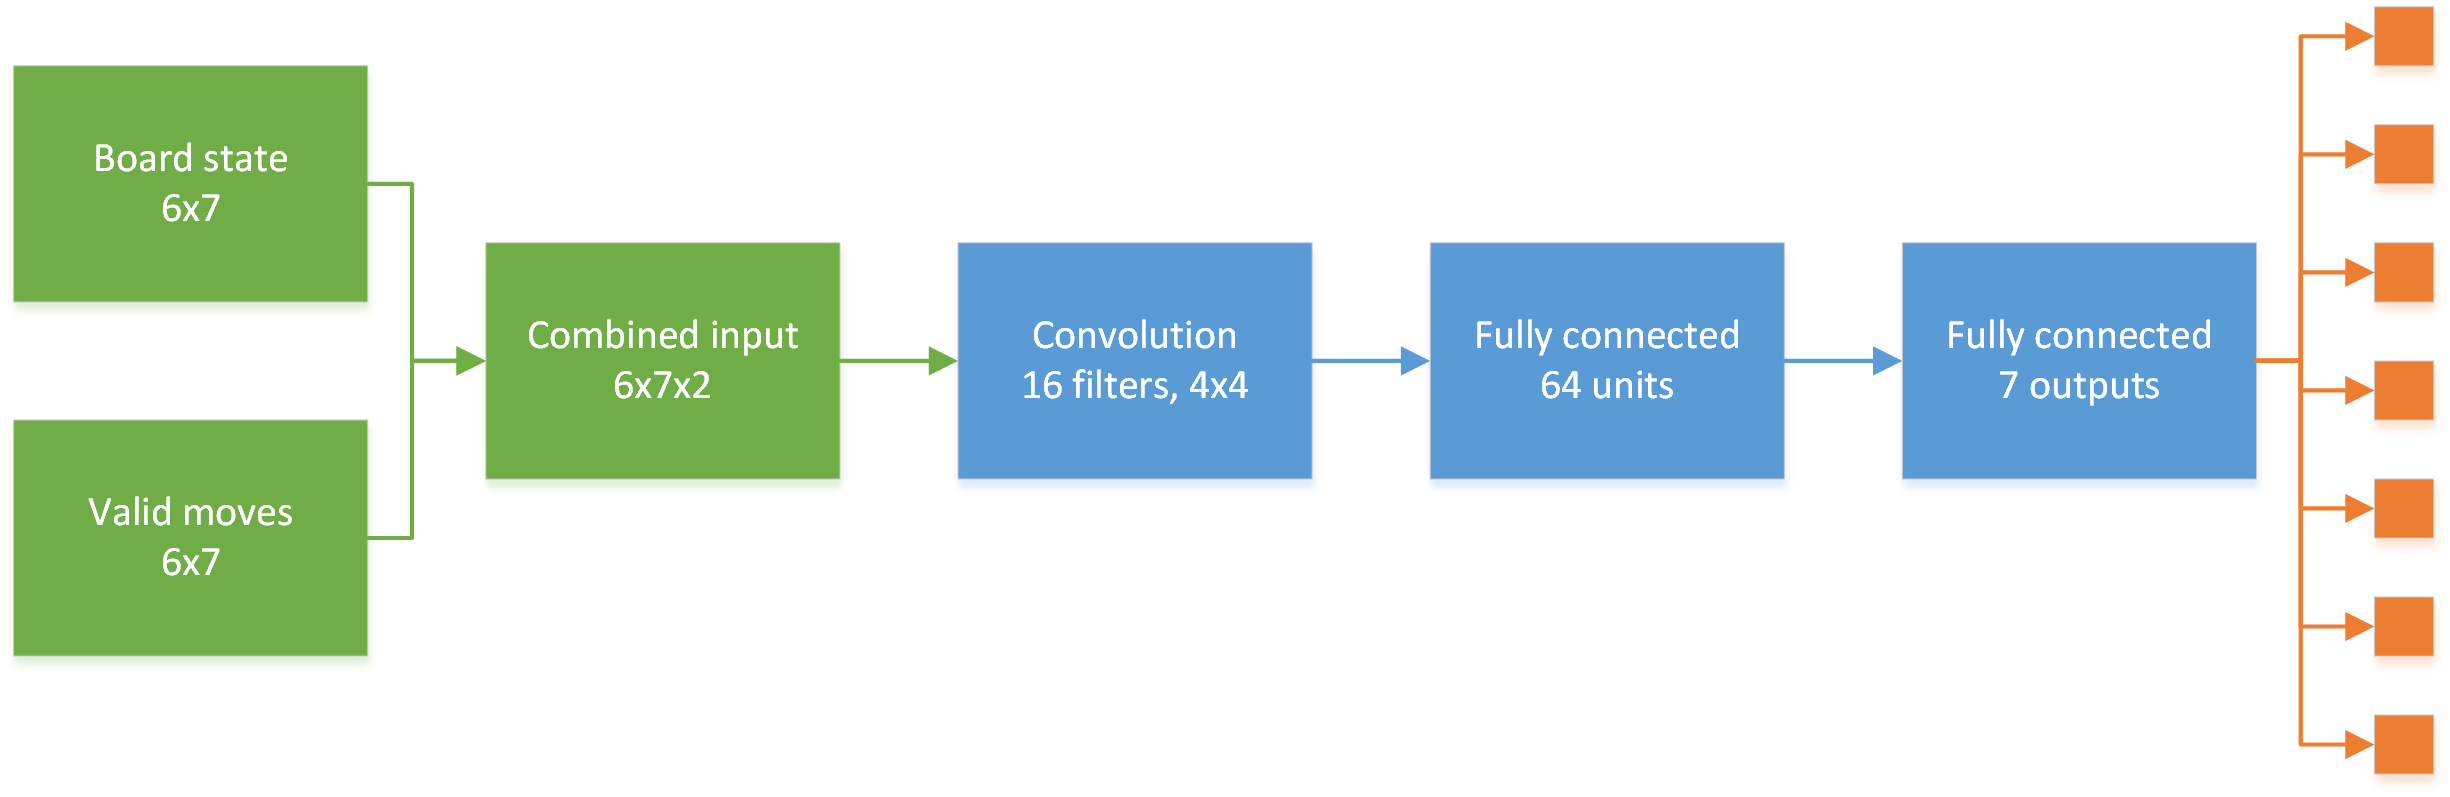
\includegraphics[width=\linewidth]{Network1.png}
  \caption{Possible future network structure}
  \label{fig:struct_future}
\end{figure}

This is just another structure that we could try. Additional structures with more layers could be used to create a better network. 

Finally, we would like to attempt to incorporate memory. Just like a person will try to manipulate the game to get to a state where they know they can win, we want to add that ability to the network. By giving a board state to the network which is close to our current board state and a state from which we have won before we could train the network to use the memory of past games to improve future games performance just like a person would do.